\documentclass[]{article}
\usepackage[OT4]{polski}
\usepackage[utf8]{inputenc}
\usepackage{graphicx}
\usepackage{float}
\usepackage{geometry}
\usepackage{xcolor}
\usepackage{caption}
\usepackage{subcaption}

\title{Projekt zaliczeniowy\\Języki Skryptowe\\"Licznik Znaków"}
\author{Artur Bednarczyk\\Politechnika Śląska\\Wydział Matematyki Stosowanej\\Informatyka, semestr III}
\date{Styczeń 2018}

\begin{document}

\maketitle
\begin{figure}[H]
	\centering
	
\includegraphics[width=0.5\linewidth]{LOGO}
	\label{fig:logo}
\end{figure}
\clearpage
\tableofcontents
\clearpage

\section{Opis zadania}
Celem zadania jest utworzenie skryptu systemowego, który będzie pełnił rolę menu. Menu powinno posiadać opcje takie jak utworzenie nowego raportu, utworzenie kopii zapasowej istniejącego raportu, wyjście. Nowy raport będzie generowany poprzez skrypt Python, na podstawie plików wyjściowych utworzonych przez aplikację napisaną w dowolnym języku programowania, która zlicza liczbę wystąpień znaków w plikach tekstowych, które są traktowane jako pliki wejściowe tej aplikacji.

\section{Algorytm}
\subsection{Opis}
Po uruchomieniu skryptu systemowego ukazuje się menu, którego opcjami są: generowanie nowego raportu, kopia zapasowa istniejącego raportu, wyśjcie. Po wybraniu opcji "wyjście" skrypt kończy pracę i nic wiecej się nie dzieje. Po wybraniu opcji "kopia zapasowa" skrypt sprawdza czy isnieje kopia zapasowa, jeśli tak to wyświetla komunikat, że istnieje, jeśli nie to tworzy nową kopię. Kopia zapasowa posiada w nazwie datę oraz godzinę wykonania, na podstawie której jest sprawdzanie czy istnieje. Po wybraniu opcji opcji "utwórz nowy raport", dla każdego pliku wejściowego wykona się program zliczający i na wyjściu da plik z liczbą znaków. Na podstawie tych plików wyjściowych Python generuje raport.
\subsection{Schemat blokowy}
\begin{figure}[H]
	\centering
	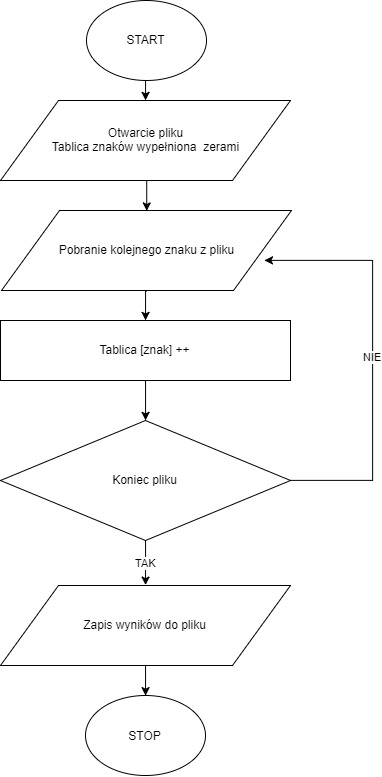
\includegraphics[width=0.5\linewidth]{scheme_diagram}
	\caption{Schemat Blokowy}
	\label{fig:schemeDiagram}
\end{figure}
\section{Implementacja}
\subsection{Batch}
\begin{figure}[H]
	\centering
	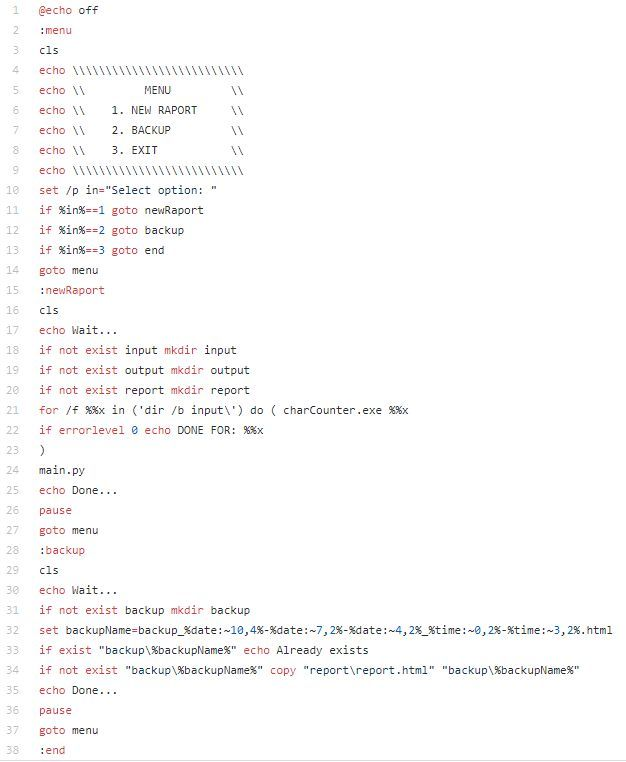
\includegraphics[width=0.9\linewidth]{batch_code}
	\caption{Kod Batch}
	\label{fig:batchcode}
\end{figure}

\subsection{C++}
\begin{figure}[H]
	\centering
	\begin{subfigure}{.5\textwidth}
		\centering
		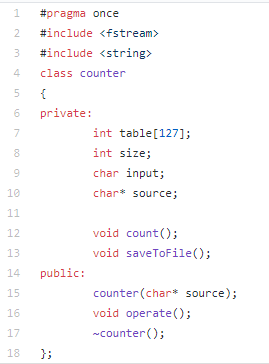
\includegraphics[width=0.7\linewidth]{h_code}
		\caption{.h}
		\label{fig:sub1}
	\end{subfigure}%
	\begin{subfigure}{.5\textwidth}
		\centering
		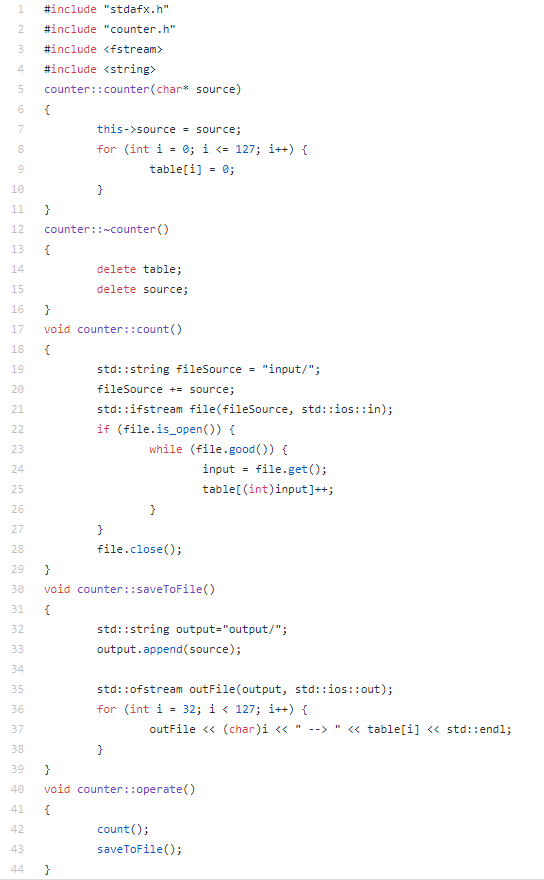
\includegraphics[width=1.3\linewidth]{cpp_code}
		\caption{.cpp}
		\label{fig:sub2}
	\end{subfigure}
	\caption{Kod C++}
	\label{fig:test}
\end{figure}
Utworzone funkcje counter() oraz saveToFile() są odpowiedzialne odpowiednio za zliczanie znaków oraz zapis wyników do pliku. Liczba wystąpień danego znaku przechowywana jest w tablicy.
\subsection{Python}
\begin{figure}[H]
	\centering
	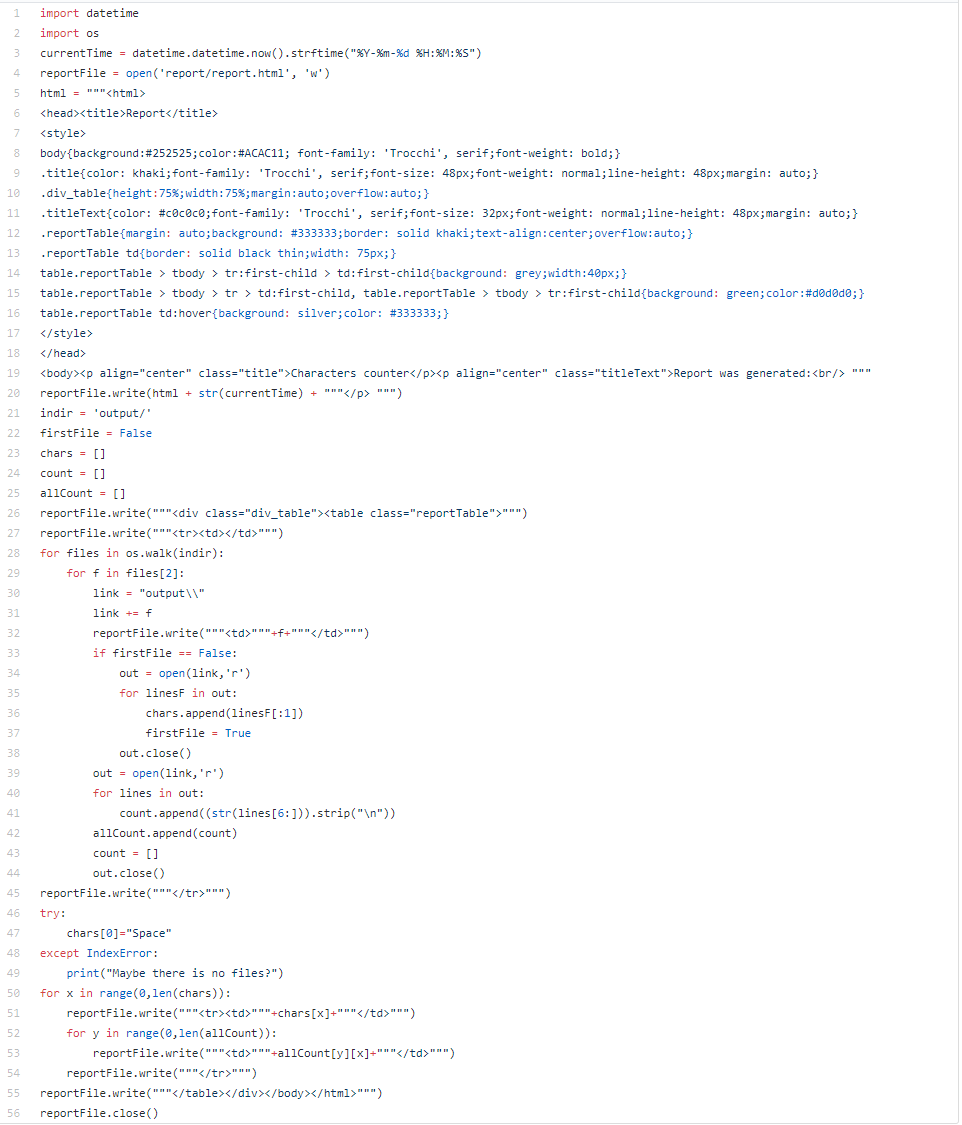
\includegraphics[width=1\linewidth]{python_code}
	\caption{Kod Python}
	\label{fig:pythoncode}
\end{figure}
\section{Działanie}
\subsection{Schemat serwera}
\begin{figure}[H]
	\centering
	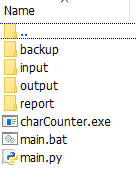
\includegraphics[width=0.4\linewidth]{folders}
	\caption{Foldery}
	\label{fig:folders}
\end{figure}
W folderze input znajdują się pliki wejściowe, czyli pliki, w których będą zliczane znaki. W folderze output znajdują się wyniki obliczeń. Folder backup zawiera kopie zapasowe raportów, a w folderze report znajduje się ostatni wykonany raport.
\begin{figure}[H]
	\centering
	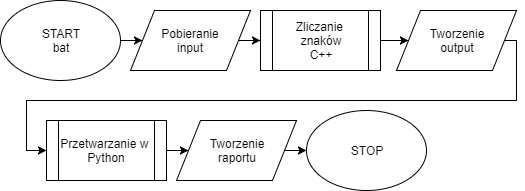
\includegraphics[width=0.9\linewidth]{flowchart}
	\caption{Flowchart}
	\label{fig:flowchart}
\end{figure}
\subsection{Prezentacja wyników}
\begin{figure}[H]
	\centering
	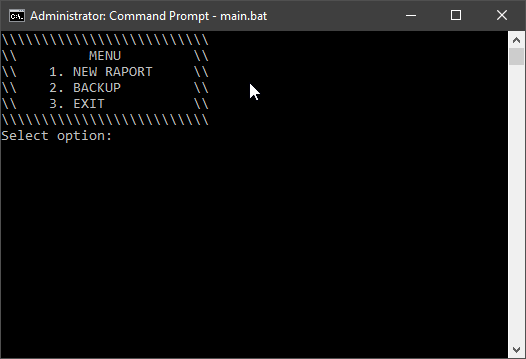
\includegraphics[width=0.7\linewidth]{prezentacja_1}
	\caption{Menu}
	\label{fig:p1}
\end{figure}
\begin{figure}[H]
	\centering
	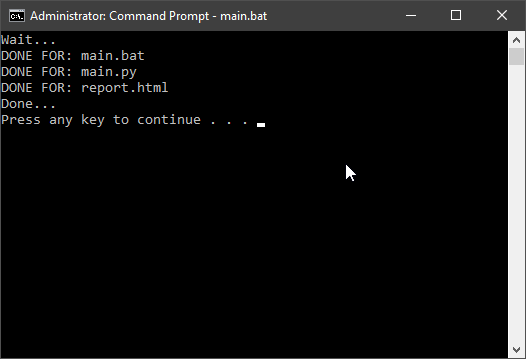
\includegraphics[width=0.7\linewidth]{prezentacja_2}
	\caption{Nowy raport}
	\label{fig:p2}
\end{figure}
\begin{figure}[H]
	\centering
	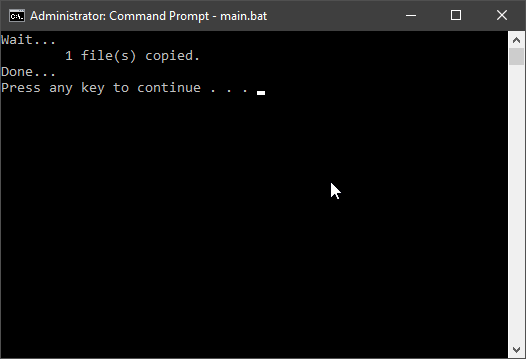
\includegraphics[width=0.7\linewidth]{prezentacja_3}
	\caption{Kopia zapasowa}
	\label{fig:p3}
\end{figure}
\begin{figure}[H]
	\centering
	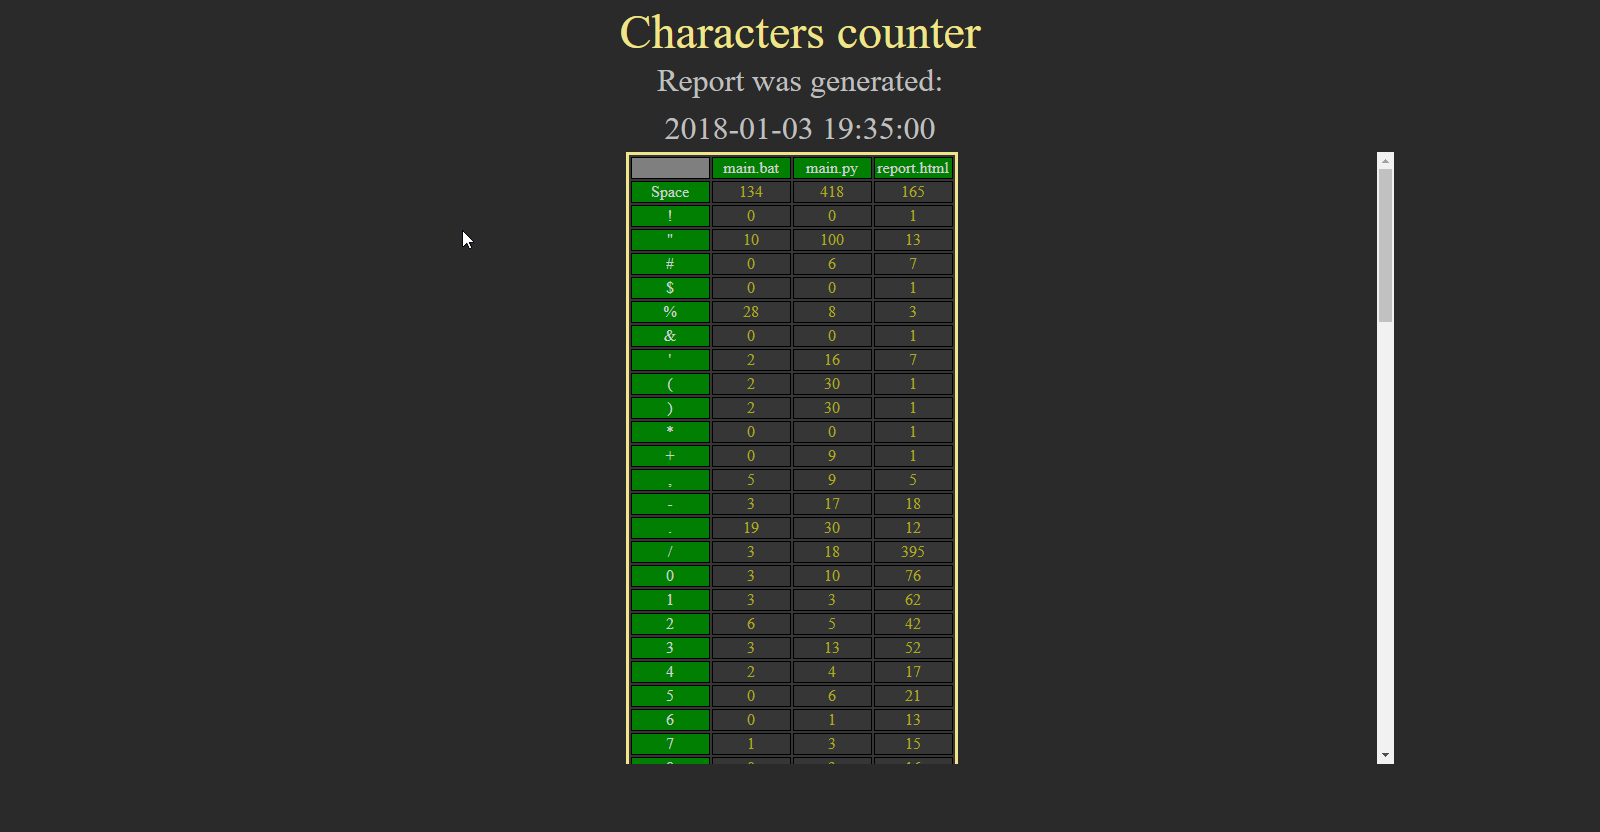
\includegraphics[width=1\linewidth]{report}
	\caption{Przykładowy raport}
	\label{fig:report}
\end{figure}\clearpage
\section{Testy}
W ramach testów, były usuwane foldery, pliki wejściowe. Przeprowadzone testy, pozwoliły na zabezpieczenie projektu przed problemami z brakującymi plikami. Gdy użytkownik usunie jakiś folder, zostanie on utworzony podczas działania skryptu.
\section{Podsumowanie}
\subsection{O projekcie}
Projekt został wykonany z wykorzystaniem:
\begin{itemize}
\item Windows 10
\item Python 3.5
\item C++ (Microsoft Visual Studio 2017 Enterprise)
\item HTML + CSS
\end{itemize}
\subsection{Przyszłość}
W przyszłości projekt może zostać rozwinięty o obsługę innych znaków, dodatkowe statystyki, wyszukiwarkę w raporcie.




\end{document}          
